\section{Methodology}
\label{sec:meth}
This section is specifically aimed at explaining how the differences in performance between a CNN-classifier and other methods are measured. This entails that the data, the experiments and the algorithms are all examined in order to show how the research question is answered. \\


\subsection{Description of the data}
\label{subsec:data}
The data used within this project consist of two types of data, both from the government of the Netherlands. The first set consists of over 50,000 questions with answers that have been asked within the Dutch national parliament. The content of these question ranges from critical examination of proposed laws to requests of more information about ongoing affairs currently within the news.\\ 

\begin{figure}[H]
	\begin{center}
		\belowbaseline[0pt]{ 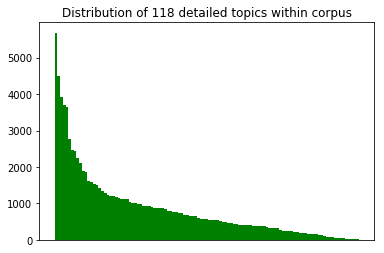
\includegraphics[width=.49\linewidth]{TrainLabels118}}~\belowbaseline[0pt]{ 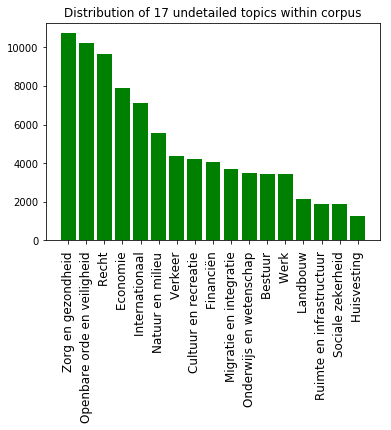
\includegraphics[width=.49\linewidth]{TrainLabels17}}
		\caption{Distribution of labels within the parlement data}
		\label{fig:distributiontopics}
	\end{center}
\end{figure}

Each question-answer pair is annotated with a number of labels. Each of the labels then consists of two levels of detail; it has one of the 17 undetailed labels, such as law or education, and one of the 118 more detailed labels, such as criminal law or primary education. Figure \ref{fig:distributiontopics} shows the distributions of labels within the dataset and figure \ref{fig:LabelAmount} shows how many labels each document contains.\\

\begin{figure}[H]
	\centering
  	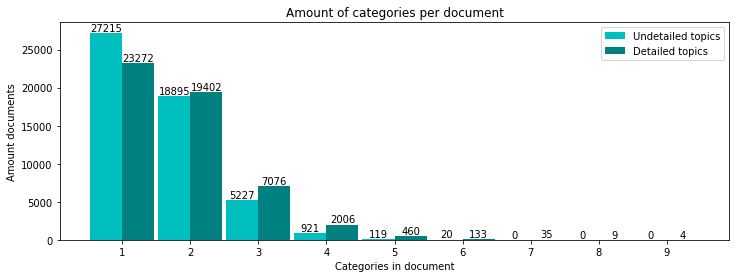
\includegraphics[width=.9\linewidth]{TrainAmountLabels}
  	\caption{Amount of labels per document}
  	\label{fig:LabelAmount}
\end{figure}

The questions are collected from www.zoek.officielebekendmakingen.nl with a scraper and the set consist of all question asked from 2001 to 2017. This means all of the labels have been discussed in many debates and varieties. Moreover, the documents vary on length as can be seen in Figure \ref{fig:WordAmount} and which politicians have asked and answered these questions.\\

\begin{figure}[H]
	\centering
  	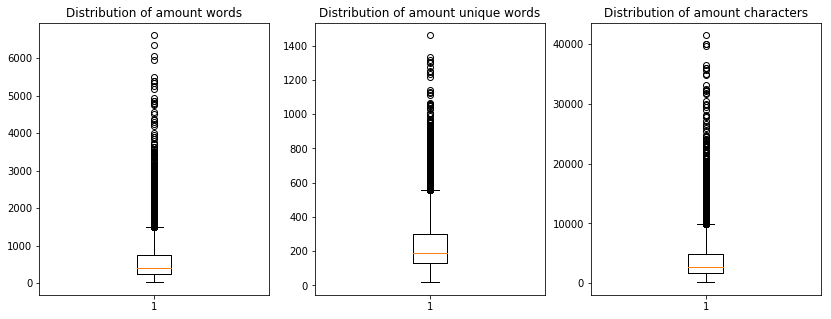
\includegraphics[width=.9\linewidth]{TrainAmountWords}
  	\caption{Box plots of the amount of words, unique words and characters within the train data.}
  	\label{fig:WordAmount}
\end{figure}

The second part of the data is retrieved from www.zoek.openraadsinformatie.nl, which contains documents of Dutch municipalities. These municipality documents consist of all kind of documents produced within municipalities, such as items on the agenda and notifications of commissions. These too have a great variety in content which ranges from discussion about local infrastructure to the re-allocation of local sport clubs. \\

\begin{figure}[H]
	\begin{center}
		\includegraphics[width=.9\linewidth]{MunLabels17}
		\caption{Distribution of labels within the municipality data}
		\label{fig:MunLabels17}
	\end{center}
\end{figure}

Large amounts of municipality data can be collected, but for this research just 25000 documents were used. Around 500 of these document were manually labeled using the taxonomieBeleidsagenda, which is the same taxonomy used for the Dutch parliament. However, the detailed labels have not been assigned, as these are too specific for untrained annotators. Similar to the training set, an overview of the label distribution, amount of labels and length of the labeled documents are visualized within Figures \ref{MunLabels17},\ref{MunAmountLabels} and \ref{MunAmountWords}. \\

\begin{figure}[H]
	\centering
  	\includegraphics[width=.9\linewidth]{MunAmountLabels}
  	\caption{Amount of labels per municipality document}
  	\label{fig:MunAmountLabels}
\end{figure}

\begin{figure}[H]
	\centering
  	\includegraphics[width=.9\linewidth]{MunAmountWords}
  	\caption{Box plots of the amount of words, unique words and characters within the municipality data.}
  	\label{fig:MunAmountWords}
\end{figure}

%Data verzameling en beschrijving van de data

%Hoe is de data verzameld, en hoe heb jij die data verkregen?


%Wat staat er in de data? Niet alleen maar een technisch verhaal, maar ook inhoudelijk. DE lezer moet een goed idee krijgen over de technische inhoud en wat het betekent.

\subsection{Algorithms}
The CNN of this research are compared to a number of traditional text classifiers; Support Vector Machines (SVM), Logistic Regression(LR), Random Forest (RF) and Multinominal Naive Bayes (NB). For all these implementations the input is a bag-of-words representation of the various documents. The implementation of Scikit-Learn is employed for these algorithms and the optimal hyper-parameters are chosen based on a grid-search. Moreover, since SVM, LG and NB are not suited for multilabel they are employed with a one-versus-all classifier as well. This means that per label one classifier is built which independently of the other classifiers and labels predicts whether a sample belongs to that label.  \\
The CNN within this research are similar to earlier architectures \cite{kim2014convolutional}. This means that an embedding layer is used to transform sentences to a multi-dimensional space using Word2Vec-embeddings. This research experiments with two embeddings, namely pre-trained embeddings retrieved trainedon a variety of Dutch resources \cite{tulkens2016evaluating} and embeddings trained on the data described in section \ref{subsec:data}. Both embedding spaces have been tested with static and non-static initializations. Thereafter three convolutional layers and three max-pooling layers are alternated between. For the convolutional layers multiple filter sizes have been tested and in addition also multiple filter sizes in one layer are experimented with.\\
Then the multidimensional is flattened and a dropout layer is used to prevent overfitting within the network. In some architectures also L1-regularization has been used, however, later research demonstrated the minimal effect of this regularization \cite{zhang2015sensitivity}. The last two layers are fully connected layers in order to gain the final prediction. Since the classification task is multilabel, binary crossentropy is used as loss function in combination with the sigmoid function as activation within the final dense layer \cite{nam2014large}. The output of the sigmoid function is a number between 0 and 1 per label, and multiple thresholds are tested in order to determine when to predict a certain label. All the parameters of this standard version of CNN are listed in Table \ref{ParametersCNN}\\


\begin{table}[H]
\centering
\caption{Parameter and values within standard CNN}
\label{ParametersCNN}
\begin{tabular}{@{}ll@{}}
\toprule
\textbf{Parameter}      	& \textbf{Values}                             			\\ \midrule
Word2Vec Model          	& Pre-trained, trained on corpus              		\\
Word2Vec Initialization 	& Dynamic, Static                            			\\
Amount of filters       	& 1,3                                        				\\
Filter sizes           		& 3,4,5 (combined whem amount of filters = 3) 	\\
Threshold of prediction	& 0.3,0.4,0.5,0.6,0.7                         			\\ \bottomrule
\end{tabular}
\end{table}

A different approach which deals with the length discrepancy of the documents is splitting the sentences up into smaller parts. Each of these individual parts of the sentence are classified individually. Then these predictions aggregated into one prediction, either by summing or using the max value. Then once again predictions above a certain threshold are predicted to belong to that label, and those below that threshold are considered not to have that label. All the parameters of this variation of CNN are listed in Table \ref{ParametersCNNSplit}.

\begin{table}[H]
\centering
\caption{Parameter and values within split version of CNN}
\label{ParametersCNNSplit}
\begin{tabular}{@{}ll@{}}
\toprule
\textbf{Parameter}      	& \textbf{Values}                             			\\ \midrule
Input size              		& 200, 400, 800                               			\\
Word2Vec Model          	& Pre-trained, trained on corpus              		\\
Word2Vec Initialization 	& Dynamic, Static                             			\\
Amount of filters       	& 1,3                                         				\\
Filter sizes            		& 3,4,5 (combined whem amount of filters = 3) 	\\
Aggregation             	& sum, max                                    			\\
Threshold of prediction 	& 0.3,0.4,0.5,0.6,0.7                         			\\ \bottomrule
\end{tabular}
\end{table}

%This research adds to the existing architectures in its method to deal with variable document sizes instead of merely padding and cutting sentences to the input size. Two possibilities have been examined; Firstly, the sentences are split into multiple smaller parts. Each of these individual parts of the sentence are classified individually. Then these predictions aggregated into one prediction, either by summing or using the max value. Then once again these predictions are rounded per label to create a prediction. All the parameters of the basic version of CNN are listed in Table \ref{ParametersCNN}.\\
%The second implementation attempts to fix the length discrepency within the embedding stage. The documents are all split in an equal number pieces. These pieces are then embedded using the Par2Vec embeddings \cite{le2014distributed}, which employs a pre-trained embedding space. This method ensures that all the documents have an equal input size for the network, however, for some documents the embeddings represent multiple words or even entire paragraphs. Similarly to the other classifiers, multiple parameters are tested such as input-size, static and non-static initialization and filter sizes. \\ 

\subsection{Experiments}
The various algorithms are evaluated on the basis of two test-sets, both from a different source of data as explained in section \ref{subsec:data}. The first experiment is carried out on the data with question of the Dutch parlement. This set is split into three parts of respectively 70, 20 and 10 percent of the data. The models are firstly trained on 70 percent of the data. Then, the optimal hyperparameters, such as the decision threshold, are chosen by evaluating the performance on the 20 percent of the data. When these parameters have been selected, the final versions is tested with the last 10 percent of the data. This experiment is conducted twice, using both the data with 17 and 118 different topics. Using different amount of topics shows how well algorithms perform depending on the detail of the topics.\\
Within the second experiment the transfer between different datasets is specifically important. The model is trained on 80 percent of the parlement-data and the remaining parlement data is used as validation data to select the optimal parameters. However, this model is evaluated using the manually labelled dataset of the Dutch municipalities in order to see how well the models transfer to another dataset. In contrast to the first experiment this experiment is merely conducted with 17 topics, as the municipality data is only classified that way.\\
Success in both experiments is measured using the micro-average F1-score, which balances the precision and recall of the prediction. However, in addition to the F1-scores also confusion matrices are used in order to evaluate what kind of errors are made. Lastly, properties of documents that are missclassified are evaluated per algorithm to better understand how the algorithms perform on specific types of documents. 


%Hoe je je vraag gaat beantwoorden.
%
%
%Dit is de langste sectie van je scriptie. 
%
%Als iets erg technisch wordt kan je een deel naar de Appendix verplaatsen. 
%
%Probeer er een lopend verhaal van te maken.
%
%Het is heel handig dit ook weer op te delen nav je deelvragen:
%
%\subsubsection{RQ1}
%
%\subsubsection{RQ2}